\section{Experiments}

\subsection*{Evaluation Scenario and Metrics}\begin{frame}\frametitle{Evaluation Scenario}
    \begin{itemize}
        \item Several objects enter and exit at different times, moving independently.
        \item Two objects emerge near the radar in areas where targets typically do not appear.

        \begin{center}
            \vspace*{3mm}
            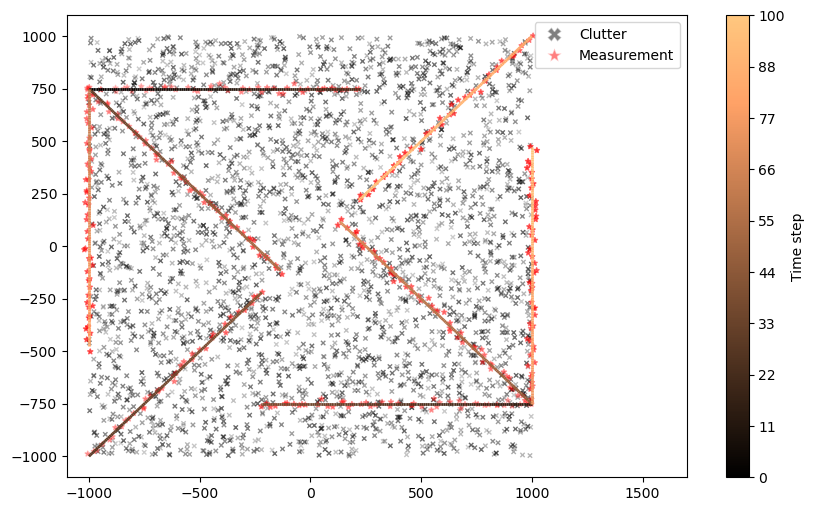
\includegraphics[width=0.6\linewidth]{pic/experiment-true.png}
        \end{center}
    \end{itemize}
\end{frame}

\begin{frame}\frametitle{Metrics}
    \begin{itemize}
        \item We'll compare the filter's performance with and without information fusion.
        \item We'll average the following metrics over 100 independent runs:
        \begin{itemize}
            \item \textbf{Circular Position Error Probability (CPEP)} — the precision error in target estimates. Lower is better.
            \item \textbf{Expected Absolute Error on the number of targets (EAE)} — the error in estimating the number of targets. Again, lower is better.
        \end{itemize}
    \end{itemize}
\end{frame}

\begin{frame}\frametitle{Experiment Results}
    \begin{center}
    \begin{tabular}{c c} 
     No Fusion & With Fusion \\ [0.1ex] 
        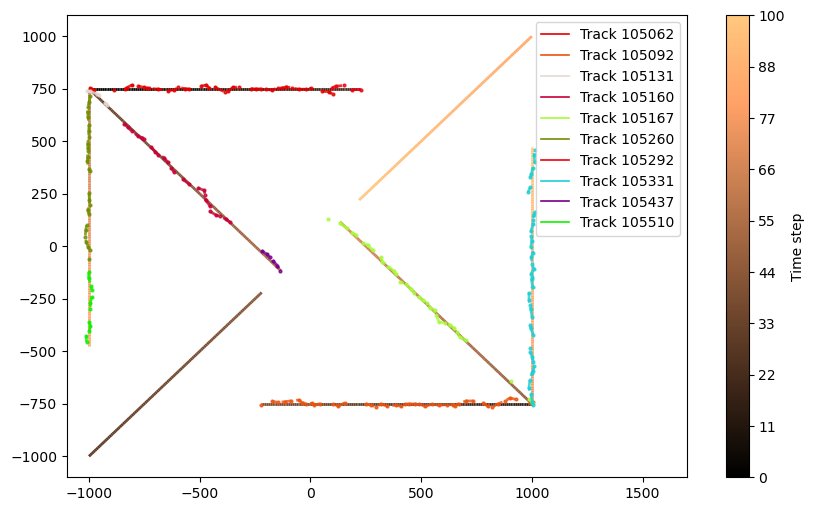
\includegraphics[width=0.45\linewidth]{pic/nf-traj.png}
    &
        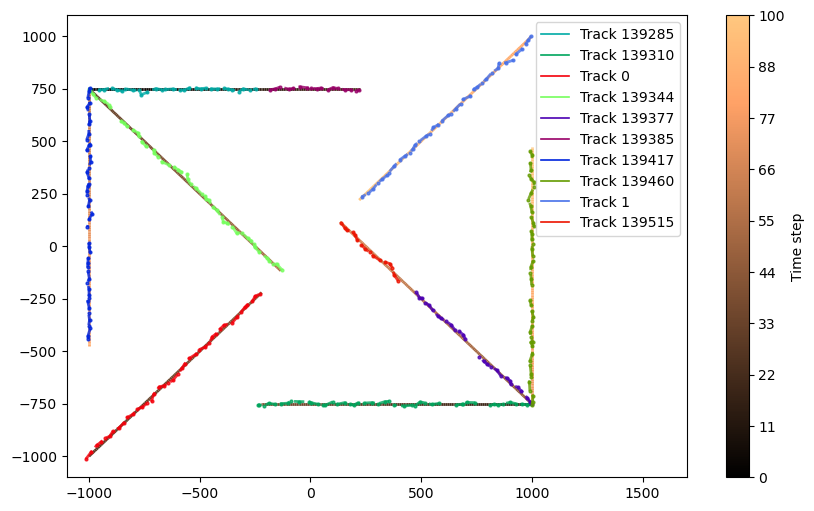
\includegraphics[width=0.45\linewidth]{pic/wf-traj.png}
    \\ [1ex]
    \end{tabular}
    \end{center}

    \begin{table}
    \begin{center}
    \begin{tabular}{ | c || c | c | }
        \hline
                & CPEP              & EAE               \\ [0.5ex]
        \hline\hline
        (NF)    & 0.87876           & 0.85900           \\ 
        (WF)    & \textbf{0.85900}  & \textbf{0.35380}  \\ [0.6ex]
        \hline
    \end{tabular}
    \end{center}
    \caption{GM-PHD filter with (WF) and without (NF) information fusion.}
    \end{table}
\end{frame}

